\documentclass[10pt,twocolumn,letterpaper]{article}

\usepackage{cvpr}
\usepackage{times}
\usepackage{epsfig}
\usepackage{graphicx}
\usepackage{amsmath}
\usepackage{amssymb}

% Include other packages here, before hyperref.

% If you comment hyperref and then uncomment it, you should delete
% egpaper.aux before re-running latex.  (Or just hit 'q' on the first latex
% run, let it finish, and you should be clear).
\usepackage[breaklinks=true,bookmarks=false]{hyperref}

\cvprfinalcopy % *** Uncomment this line for the final submission

\def\cvprPaperID{****} % *** Enter the CVPR Paper ID here
\def\httilde{\mbox{\tt\raisebox{-.5ex}{\symbol{126}}}}

% Pages are numbered in submission mode, and unnumbered in camera-ready
%\ifcvprfinal\pagestyle{empty}\fi
\setcounter{page}{4321}
\begin{document}

%%%%%%%%% TITLE
\title{Vision and Language in 3D}

\author{Yuval Atzmon\\
Bar Ilan University\\
Ramat Gan, Israel\\
{\tt\small yuval.atzmon@biu.ac.il}
% For a paper whose authors are all at the same institution,
% omit the following lines up until the closing ``}''.
% Additional authors and addresses can be added with ``\and'',
% just like the second author.
% To save space, use either the email address or home page, not both
\and
Second Author\\
Institution2\\
First line of institution2 address\\
{\tt\small secondauthor@i2.org}
}

\maketitle
%\thispagestyle{empty}

%%%%%%%%% ABSTRACT
\begin{abstract}
 We constructed a system that tracks activities in videos, given a descriptive text sentence, and outputs the likelihood of how well the description match the activity in the video. We integrated depth estimation for single-len camera, and demonstrated its ability to track 3D actions in single-len camera videos. That could not be otherwise addressed. 
 

\end{abstract}

%%%%%%%%% BODY TEXT
\section{Introduction}

TBD

\subsection{Vision and language system}

 integrates language and videos. Basically, we run an object detector on each frame, allowing many false-positive (so detection rate will be high). Now we treat the detections as the states of a generalized HMM of a tracker that gives high score for coherency between frames (we use optical flow to account for movemennt), and do inference over it (with viterbi decoder) to find the best track. 
On top of the tracker HMM there's another layer of language HMM, which biases the tracker results. In fact, we match a tracker for each noun, and do joint inference on all together. So for example a verb with 2 nouns (a person approaches a chair) will generate two trackers, one for each noun. The observations of the 1st noun will be classes of detections of the 1st tracker. The observations of the 2nd noun will be classes of detections of the 2nd tracker. The observations of verb will be the relative distances and velocities between the detetcions of both trackers.
We take the outer product of all possible states of all the HMMs and combine them to a single viterbi inference mechanism. So eventually you result with tracking on only the actions that were described in the sentence (kind of an attention mechanism), and you get a likelihood score for how well this action corresponds to the events in the video. Now since HMM are generative models, you can actually do many other tasks with this mechanism, such as generating descriptions from videos, question answering, ...

%-------------------------------------------------------------------------
\subsubsection{Integrating depth estimation}
TBD

\subsection{Results}
TBD


%in~\cite{Authors14b}''.  Then submit the techreport as additional material.


\begin{figure}[t]
\begin{center}
%\fbox{\rule{0pt}{2in} \rule{0.9\linewidth}{0pt}}
   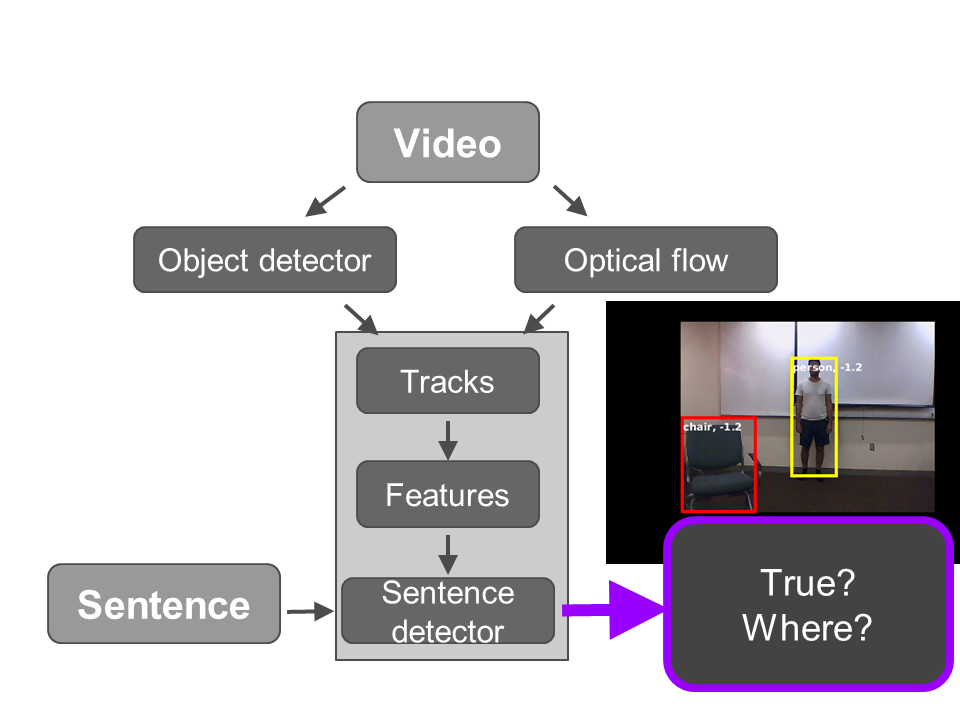
\includegraphics[width=0.8\linewidth]{system_overview.png}
\end{center}
   \caption{System overview}
\label{fig_system}
\end{figure}

\subsection{Miscellaneous}

\noindent
Compare the following:\\
\begin{tabular}{ll}
 \verb'$conf_a$' &  $conf_a$ \\
 \verb'$\mathit{conf}_a$' & $\mathit{conf}_a$
\end{tabular}\\
See The \TeX book, p165.

TBD

\begin{figure*}
\begin{center}
%\fbox{\rule{0pt}{2in} \rule{.9\linewidth}{0pt}}
   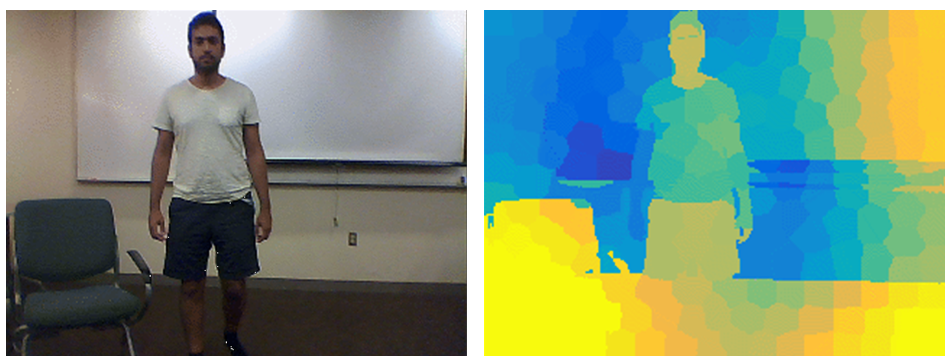
\includegraphics[width=0.8\linewidth]{depth_estim_example.png}
   \end{center}
   \caption{Example for depth estimation in a single frame}
\label{fig_depth_frame}
\end{figure*}

TBD

\begin{figure*}
\begin{center}
%\fbox{\rule{0pt}{2in} \rule{.9\linewidth}{0pt}}
   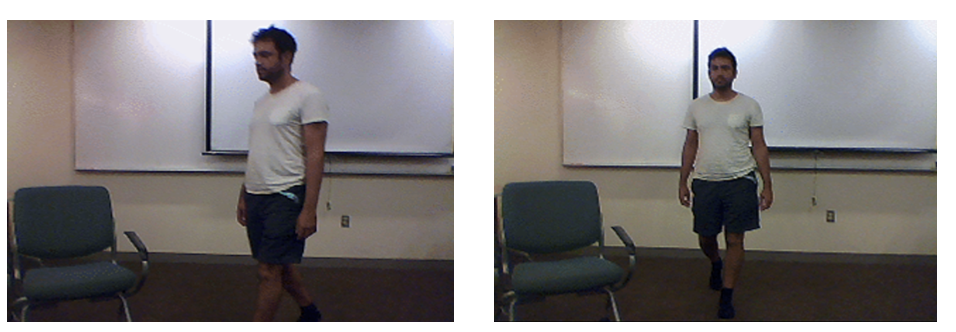
\includegraphics[width=0.8\linewidth]{front_vs_side_approach.png}
   \end{center}
   \caption{"A person approaches a chair": frontal vs side approach}
\label{fig_front_vs_side}
\end{figure*}


{\small
\bibliographystyle{ieee}
\bibliography{egbib}
}

\end{document}
